\documentclass[11pt]{article}

\usepackage{graphicx}
\usepackage[top=25mm, bottom=25mm, left=25mm, right=25mm, a4paper]{geometry}
\usepackage{amsmath}
\usepackage{enumitem}
\usepackage{float}
\usepackage{fancyhdr}
\usepackage{booktabs}
\usepackage{tikz}
\usepackage{steinmetz}

\pagestyle{fancy}
\fancyhf{}
\fancyhead[R]{Baturay Kafkas - 2240357068 - Electrical \& Electronics Engineering}

\rfoot{\thepage}
\renewcommand{\headrulewidth}{0pt} 
\renewcommand{\footrulewidth}{0pt}
\sloppy

\begin{document}

\begin{center}
\large
\textbf{ELE214 - Electronics Laboratory I Preliminary Work 6}
\end{center}

\section{Questions}

\begin{enumerate}[leftmargin=*,label=\textbf{\arabic*.}]

\item Determine the range in which the MOSFET is employed as an amplifier. Comment on whether the MOSFET is ON or OFF in this range. 

\item Calculate the appropriate $R_{P1}$ (constant) value for the $V_\text{out}$ voltage to be $7.5$ V and explain it in detail. Also, find the voltage gain of the circuit. Take $V_\text{in}=50\sin(\omega t)$ mV, at $100$~Hz.

\textbf{Computer Assignment: Simulate 1-2.}

\end{enumerate}

\begin{figure}[H]
    \centering
    
\includegraphics[width=0.5\linewidth]{fig1.png}
    
    \textit{Figure 1: Circuit diagram}
\end{figure}

\textbf{Experimental Work}

\begin{enumerate}[leftmargin=*,label=\textbf{\arabic*.}]

\item Set up the circuit in \textit{Figure 1}. Adjust the potentiometer to obtain the output voltage of $4$~V, $7.5$~V, and $11$~V (measure the $V_\text{out}$ using a multimeter). Repeat steps $2$ and $3$ for $V_\text{out}=4$~V, $V_\text{out}=7.5$~V, and $V_\text{out}=11$~V.

\item Measure the $V_{GS}$ value of the MOSFET.

\item Determine the voltage gain. Take $V_\text{in}=50\sin(\omega t)$~mV at $100$~Hz.

\end{enumerate}

\section{Answers}

\begin{enumerate}[leftmargin=*,label=\textbf{\arabic*.}]

\item For the MOSFET to be used as an amplifier, it should be in the saturation mode. In this mode, the MOSFET is ON. Impose the condition for saturation:
\[V_{DS}\ge V_{GS}-V_{TH},\]

where $V_{DS}$ is the drain-source voltage, $V_{GS}$ is the gate-source voltage and $V_{TH}$ is the threshold voltage.

\item From the previous experiment, the 2N7000 transistor is presumed to be used in this experiment as well. Since the value $K=\frac12\mu_nC_{ox}\frac{W}{L}$ is unknown, we can consider the value from LTspice.
\[K=0.085\]

DC analysis of the circuit:

\begin{minipage}{0.37\textwidth}
\begin{figure}[H]
    \centering
    
\includegraphics[width=1\linewidth]{fig2.png}
    
    \small \textit{Figure 2: DC Analysis}
\end{figure}
\end{minipage}\hfill\begin{minipage}{0.57\textwidth}
To make sure $V_{GS}>V_{TH}$, inspect the $G-S$ loop.
\[V_{G}=V_{1}\cdot\frac{R_{P1}}{R_1+R_{P1}},\quad V_S=0~\text{V}\]
\[V_{GS}>V_{TH}\implies V_G-V_S=V_1\cdot\frac{R_{P1}}{R_1+R_{P1}}-0>V_{TH}\]
\[\implies 15R_{P1}>1.6R_{P1}+1.6R_1\implies13.4R_{P1}>1.6R_1\]
\[\implies R_{P1}>\frac{1.6}{13.4}R_1\approx39.4~\text{k}\Omega\]
\end{minipage}

\vspace{1em}

Inspect the $D-S$ loop:
\[V_1-I_D\cdot R_2-V_{DS}=0,\quad V_{DS}\ge V_{GS}-V_{TH}\implies V_1-I_D\cdot R_2\ge V_{GS}-V_{TH}\]
\[\implies V_1\ge KR_2(V_{GS}-V_{TH})^2+V_{GS}-V_{TH}\implies 85(V_{GS}-1.6)^2+V_{GS}-1.6\le15\]
\[85V_{GS}^2-271V_{GS}+201\leq0\implies 1.174 ~\text{V} \le V_{GS}\le2.014~\text{V}\]
\[\implies 1.174\le V_1\cdot\frac{R_{P1}}{R_1+R_{P1}}\le 2.014\implies 28.2~\text{k}\Omega \le R_{P1} \le 51.0~\text{k}\Omega
\]

\[V_{GS}>V_{TH}\quad\&\quad V_{DS}\ge V_{GS}-V_{TH}\implies\boxed{39.4~\text{k}\Omega \le R_{P1} \le 51.0~\text{k}\Omega}\]

We want to achieve $V_\text{out}=7.5$~V.
\begin{align*}V_\text{out}&=V_{DS}=V_1-I_D\cdot R_2=V_1-KR_2\left(V_1\cdot\frac{R_{P1}}{R_1+R_{P1}}-V_{TH}\right)^2\\&=15-0.085\cdot1000\left(15\cdot\frac{R_{P1}}{330000+R_{P1}}-1.6\right)^2=7.5\end{align*}
\[\implies R_{P1,1}\approx 31.34~\text{k}\Omega,\quad R_{P1,2}\approx 47.74~\text{k}\Omega\]

Since $31.34$~k$\Omega$ is out of range, $\boxed{R_{P1}=47.74~\text{k}\Omega}$.

Small-signal AC analysis of the circuit:

\begin{figure}[H]
    \centering
    
\includegraphics[width=0.75\linewidth]{fig3.png}

    \small \textit{Figure 3: Small-Signal AC Analysis}
\end{figure}

\[A_v=\frac{V_\text{out}}{V_\text{in}}=\frac{-g_mV_{GS}R_2}{V_{GS}}=-2K(V_{GS}-V_{TH})R_2=-2K\left(V_{1}\cdot\frac{R_{P1}}{R_1+R_{P1}}-V_{TH}\right)R_2\]
\[A_v=-2\cdot0.085\left(15\cdot\frac{47.74~\text{k}}{330\text{ k}+47.74~\text{k}}-1.6\right)\cdot1000\approx\boxed{-50.29}\]
\end{enumerate}

\textbf{Simulation}

\begin{enumerate}[leftmargin=*,label=\textbf{\arabic*.}]

\item The circuit:

\begin{minipage}{0.46\textwidth}
\begin{figure}[H]
    \centering
    
\includegraphics[width=1\linewidth]{fig4.png}
    
    \small \textit{Figure 4: Circuit Diagram}
\end{figure}
\end{minipage}\hfill\begin{minipage}{0.46\textwidth}
\begin{figure}[H]
    \centering
    
\includegraphics[width=1\linewidth]{fig5.png}
    
    \small \textit{Figure 5: Graph for Different Values of} $R_{P1}$
\end{figure}
\end{minipage}

\vspace{1em}

\item From \textit{Figure 5}, we can observe that for $V_\text{out}=7.5$~V, the value of the resistor should be $R_{P1}\approx47.94$~k$\Omega$.

\begin{minipage}{0.46\textwidth}
\begin{figure}[H]
    \centering
    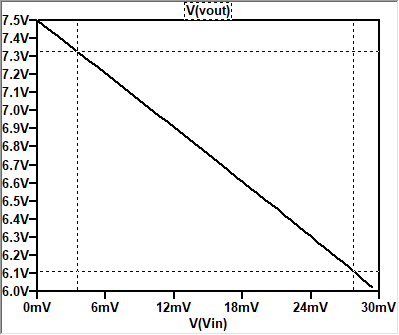
\includegraphics[width=1\linewidth]{fig6.png}

    \small \textit{Figure 6: Circuit Behavior for 1 Milisecond}
\end{figure}
\end{minipage}\hfill\begin{minipage}{0.46\textwidth}
\begin{figure}[H]
    \centering
    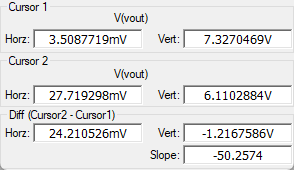
\includegraphics[width=1\linewidth]{fig7.png}

    \small \textit{Figure 7: Gain (Slope) Obtained from Figure 6}
\end{figure}
\end{minipage}

\end{enumerate}

\end{document}